\documentclass[11pt,a4paper]{article}

% ---------------------------------------------------------------
% Packages (same set-up as the THM model report)
% ---------------------------------------------------------------
\usepackage[T1]{fontenc}
\usepackage[utf8]{inputenc}
\usepackage{lmodern}
\usepackage[a4paper,margin=2.5cm]{geometry}
\usepackage{amsmath,amssymb,bm}
\usepackage{booktabs,tabularx,array}
\usepackage{siunitx}
\usepackage{enumitem}
\usepackage{xcolor}
\usepackage{graphicx}
\usepackage[numbers,sort&compress]{natbib}
\usepackage[colorlinks=true,linkcolor=blue!50!black,citecolor=blue!50!black,urlcolor=blue!50!black]{hyperref}

\sisetup{range-phrase=--, range-units=single}
\newcolumntype{L}{>{\raggedright\arraybackslash}X}
\renewcommand{\arraystretch}{1.2}
\graphicspath{{./figures/}}
\newcommand{\open}{$\square$}

% ---------------------------------------------------------------
\title{GREAT Cell Modelling Specification\\[0.5ex]
\large DECOVALEX 2027 -- SAFENET-2}
\author{Olaf Kolditz$^{1,2}$, Mostafa Mollaali$^{3,1}$\\[2ex]
\small $^{1}$Helmholtz Centre for Environmental Research -- UFZ, Leipzig, Germany\\
\small $^{2}$Technische Universit\"at Dresden, Germany\\
\small $^{3}$Technische Universit\"at Bergakademie Freiberg (TUBAF), Germany}
\date{8 November 2026}

\begin{document}
\maketitle

\begin{abstract}
This specification fixes geometry, material parameters, loads, boundary
conditions and outputs for modelling the GREAT cell experiments, so that all
DECOVALEX SAFENET-2 teams simulate the same problem and their results can be
compared directly. It is code-independent. OpenGeoSys (OGS) reference solutions
exist for the cases M1 and THM2.
\end{abstract}

\tableofcontents

% ---------------------------------------------------------------
\section{Purpose and scope}
% ---------------------------------------------------------------
\begin{itemize}
  \item \textbf{Fixed:} everything in Sections~\ref{sec:geometry} to
        \ref{sec:outputs}. Deviations must be reported.
  \item \textbf{Free:} numerical method, element type, mesh, time stepping and
        solver, within the accuracy targets of Section~\ref{sec:verification}.
  \item \textbf{Units:} SI throughout (m, s, Pa, K, kg). Strains as fractions;
        plots may use $10^{-2}$\,\%.
  \item \textbf{Model dimension:} 2D plane strain, horizontal mid-section of
        the sample, unit thickness \SI{1}{m}. All rates are per metre thickness.
\end{itemize}

% ---------------------------------------------------------------
\section{Benchmark matrix}
% ---------------------------------------------------------------
The benchmarks add one process at a time: mechanics (M), then fluid flow (HM),
then heat (THM), each for an intact sample, a single fracture and a fracture
network (Fig.~\ref{fig:concept}, Table~\ref{tab:matrix}). This version
specifies \textbf{M1} and \textbf{THM2} in full; the fractured cases follow the
same conventions and are added later.

\begin{figure}[htbp]
\centering
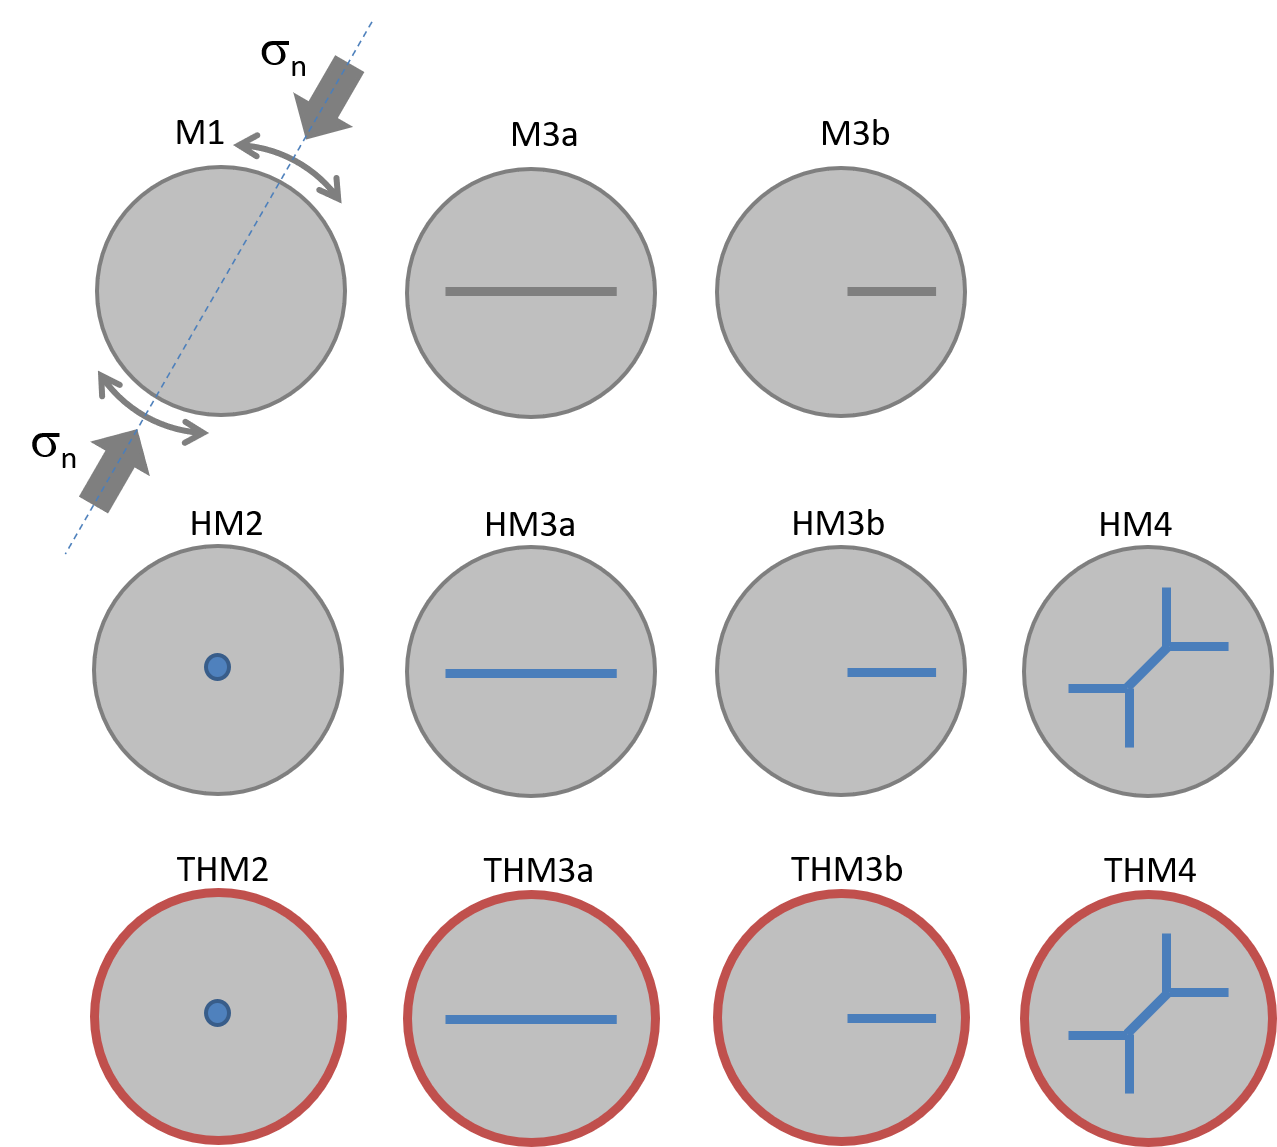
\includegraphics[width=0.6\textwidth]{great-benchmarking-thm.png}
\caption{GREAT cell benchmark concept: M (grey), HM (blue, fluid injection) and
THM (red boundary, heating) for intact, fractured and networked samples.}
\label{fig:concept}
\end{figure}

\begin{table}[htbp]
\centering
\caption{Benchmark cases.}
\label{tab:matrix}
\begin{tabularx}{\textwidth}{@{}llLL@{}}
\toprule
Case & Sample & Processes & Status \\
\midrule
M1                 & Intact                  & Poly-axial load, rotated (Loads A, E, B, F, C) & Specified; OGS reference \\
M3a / M3b          & Full / half fracture    & Mechanics                                        & Geometry given; load as M1 \\
HM2                & Intact, central borehole & Load + injection                                & Covered by THM2 without heating \\
HM3a / HM3b        & Full / half fracture    & Load + injection into fracture                   & To be specified \\
HM4                & Fracture network        & Load + injection                                 & To be specified \\
THM2               & Intact                  & Load A + heating + cold-water injection          & Specified; OGS reference \\
THM3a/b, THM4      & Fractured               & As HM3/HM4 + heating                             & To be specified \\
\bottomrule
\end{tabularx}
\end{table}

Teams are encouraged to run the stepwise sequence T $\rightarrow$ TH
$\rightarrow$ THM used for the reference model, since each step has its own
check.

% ---------------------------------------------------------------
\section{Geometry and conventions}
\label{sec:geometry}
% ---------------------------------------------------------------
The domain is a disc of radius \SI{0.100}{m} centred at $(0,0)$: rock inside
$r=\SI{0.097}{m}$ and a \SI{3}{mm} rubber sheath outside it
(Fig.~\ref{fig:geometry}, Table~\ref{tab:geometry}). Angles $\theta$ are
measured counter-clockwise from the $+x$ axis.

\begin{figure}[htbp]
\centering
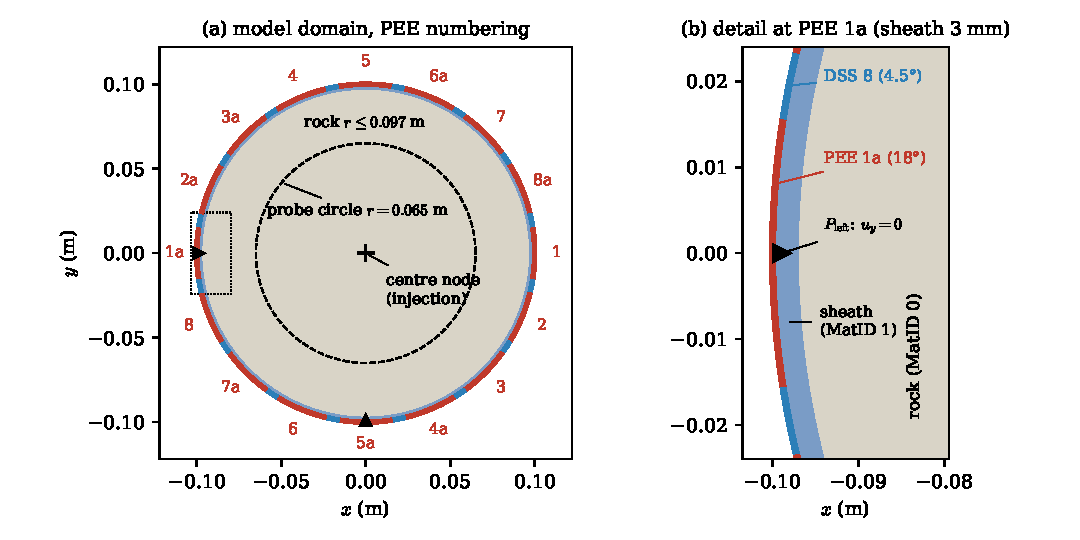
\includegraphics[width=\textwidth]{fig_geometry.pdf}
\caption{Geometry and PEE numbering (a), detail of the sheath at PEE~1a (b).}
\label{fig:geometry}
\end{figure}

\begin{table}[htbp]
\centering
\caption{Geometry and conventions.}
\label{tab:geometry}
\begin{tabularx}{\textwidth}{@{}lL@{}}
\toprule
Item & Specification \\
\midrule
Rock               & $r \le \SI{0.097}{m}$ (material 0) \\
Sheath             & $\SI{0.097}{m} < r \le \SI{0.100}{m}$ (material 1) \\
Centre point       & $(0,0)$; injection point (THM2), borehole not resolved \\
Probe circle       & $r=\SI{0.065}{m}$; volumetric strain output \\
PEE arcs           & 16 arcs of \ang{18} on $r=\SI{0.100}{m}$. PEE $i$ centred at $\theta=-(i-1)\cdot\ang{22.5}$ ($i=1\ldots8$, clockwise from $+x$); PEE $i$a opposite, at $+\ang{180}$ \\
DSS arcs           & 16 arcs of \ang{4.5} between the PEEs. DSS $i$ lies between PEE $i$ and PEE $i+1$; DSS~8 between PEE~8 and PEE~1a \\
Rigid-body control & $P_\mathrm{bottom}=(0,\,-0.09894)$\,m: $u_x=u_y=0$. $P_\mathrm{left}=(-0.09894,\,0)$\,m: $u_y=0$ \\
Full fracture (M3a/HM3a) & Segment $(-0.094,\,0.094)\,\mathrm{m}\times\{0\}$ \\
Half fracture (M3b/HM3b) & Segment $(0,\,0.04)\,\mathrm{m}\times\{0\}$ \\
\bottomrule
\end{tabularx}
\end{table}

The PEE and DSS arc widths (\ang{18}/\ang{4.5}) are estimates from Fig.~4b
of~\cite{Mollaali2026}; teams should use them until measured values are
available.

% ---------------------------------------------------------------
\section{Mesh}
% ---------------------------------------------------------------
The mesh is the team's choice, but it must resolve four features: the sheath,
the PEE/DSS arc ends, the probe circle and the centre point.
\begin{itemize}
  \item PEE/DSS arc ends and the two fixed points must be mesh nodes.
  \item The probe circle should be embedded as mesh edges, or outputs
        interpolated onto it at $\le\ang{1}$ spacing.
  \item At least two element layers across the \SI{3}{mm} sheath.
  \item Refinement towards the centre for injection; the reference uses
        $h=\SI{1.5}{mm}$ at the centre, \SI{6}{mm} at $r=\SI{0.065}{m}$ and
        \SI{2}{mm} in the sheath.
  \item Reference mesh: 11\,889 nodes, 5\,804 quadratic triangles; displacement
        quadratic, pressure and temperature linear.
\end{itemize}

% ---------------------------------------------------------------
\section{Material parameters}
% ---------------------------------------------------------------
All materials are linear elastic and isotropic. Rock values follow Table~1
of~\cite{Mollaali2026}; hydraulic and thermal values follow the reference TH
model (Table~\ref{tab:params}).

\begin{table}[htbp]
\centering
\caption{Material parameters.}
\label{tab:params}
\small
\begin{tabular}{@{}llccc@{}}
\toprule
Parameter & Unit & Greywacke & Gneiss & Sheath \\
\midrule
Young's modulus $E$                     & GPa              & 26.85 & 83.9 & 0.1 \\
Poisson's ratio $\nu$                   & --               & 0.27 & 0.21 & 0.4 \\
Solid density $\rho_s$                  & kg\,m$^{-3}$     & 2650 & 2750 & 1200 \\
Porosity $\phi$                         & --               & 0.005 & 0.001 & as rock \\
Biot coefficient $\alpha_B$             & --               & 0.8 & 0.6 & 0 \\
Permeability $k$                        & m$^2$            & \num{1.409e-14} & \num{1.409e-14} & \num{1.409e-14}$^{*}$ \\
Bulk thermal conductivity $\lambda$     & W\,m$^{-1}$\,K$^{-1}$ & 2.8 & 2.8 & 2.8 \\
Bulk heat capacity $\rho c$             & J\,m$^{-3}$\,K$^{-1}$ & \num{2.133e6} & \num{2.133e6} & \num{2.133e6} \\
Linear thermal expansion $\alpha_T$ (solid) & K$^{-1}$     & \num{8e-6} & \num{8e-6} & \num{8e-6} \\
\bottomrule
\multicolumn{5}{@{}l}{\footnotesize $^{*}$ See open items (Section~\ref{sec:open}).}
\end{tabular}
\end{table}

\textbf{Water:} $\rho_f=\SI{1000}{kg\,m^{-3}}$ at $p_0=\SI{1}{MPa}$,
compressibility \SI{4.4e-10}{Pa^{-1}}, $\mu=\SI{1e-3}{Pa\,s}$,
$c_f=\SI{4180}{J\,kg^{-1}\,K^{-1}}$, $\lambda_f=\SI{0.6}{W\,m^{-1}\,K^{-1}}$,
no thermal expansion. Storage follows from $\phi$, $\alpha_B$, the water
compressibility and the elasticity. Bulk $\lambda$ and $\rho c$ are prescribed;
teams back-calculate solid values for their own mixing rule.

% ---------------------------------------------------------------
\section{Mechanical load cases}
% ---------------------------------------------------------------
Each load case prescribes a compressive normal stress on the 16 PEE arcs
(Table~4 of~\cite{Mollaali2026}); PEE $i$ and PEE $i$a carry the same value.
Loads E, B, F and C are Load~A rotated clockwise by \ang{22.5}, \ang{45},
\ang{67.5} and \ang{90} (Table~\ref{tab:loads}).

\begin{table}[htbp]
\centering
\caption{PEE normal stress per load case (MPa, compression positive).}
\label{tab:loads}
\begin{tabular}{@{}lc*{8}{r}@{}}
\toprule
Load & Rotation & PEE 1 & PEE 2 & PEE 3 & PEE 4 & PEE 5 & PEE 6 & PEE 7 & PEE 8 \\
\midrule
A & \ang{0}    & 10.0 & 6.64 & 4.46 & 1.17 & 1.0  & 3.82 & 7.80 & 9.95 \\
E & \ang{22.5} & 9.95 & 10.0 & 6.64 & 4.46 & 1.17 & 1.0  & 3.82 & 7.80 \\
B & \ang{45}   & 7.80 & 9.95 & 10.0 & 6.64 & 4.46 & 1.17 & 1.0  & 3.82 \\
F & \ang{67.5} & 3.82 & 7.80 & 9.95 & 10.0 & 6.64 & 4.46 & 1.17 & 1.0  \\
C & \ang{90}   & 1.0  & 3.82 & 7.80 & 9.95 & 10.0 & 6.64 & 4.46 & 1.17 \\
\bottomrule
\end{tabular}
\end{table}

\begin{itemize}
  \item \textbf{DSS:} each DSS carries the mean of its two neighbouring PEEs,
        $\sigma_{\mathrm{DSS},i}=(\sigma_{\mathrm{PEE},i}+\sigma_{\mathrm{PEE},i+1})/2$,
        with PEE~9 $\equiv$ PEE~1.
  \item \textbf{Out-of-plane:} plane strain; no axial load is applied in 2D.
  \item \textbf{Gravity:} none (horizontal section).
  \item \textbf{Load path:} applied in the first time step and then held constant.
\end{itemize}

% ---------------------------------------------------------------
\section{THM2 scenario}
% ---------------------------------------------------------------
THM2 loads the intact sample with Load~A, heats it from the outer boundary for
\SI{4000}{s}, injects cold water at the centre for \SI{50}{s} and then shuts in
until \SI{5000}{s} (Table~\ref{tab:phases}, Fig.~\ref{fig:bc}). M1 is the same
model with only the mechanical load, evaluated at the end of the first step.

\begin{table}[htbp]
\centering
\caption{THM2 phases and boundary conditions.}
\label{tab:phases}
\small
\begin{tabularx}{\textwidth}{@{}llLLl@{}}
\toprule
Phase & Time (s) & Thermal & Hydraulic & Mechanical \\
\midrule
0           & $t=0$     & $T=T_0$ & $p=p_0$ & Load A applied \\
1 Heating   & 0--4000   & Outer boundary: 293 $\rightarrow$ \SI{363}{K} linearly over 0--325\,s, then \SI{363}{K} & $p=p_0$ on outer boundary & Load A held \\
2 Injection & 4000--4050 & As phase 1; centre point $T=\SI{293}{K}$ & Centre point: $Q=\SI{1}{l/min}$ per m $=\SI{1.667e-5}{m^3\,s^{-1}}$ per m (\SI{16.67}{g\,s^{-1}} per m) & Load A held \\
3 Shut-in   & 4050--5000 & As phase 1 & No injection & Load A held \\
\bottomrule
\end{tabularx}
\end{table}

\begin{figure}[htbp]
\centering
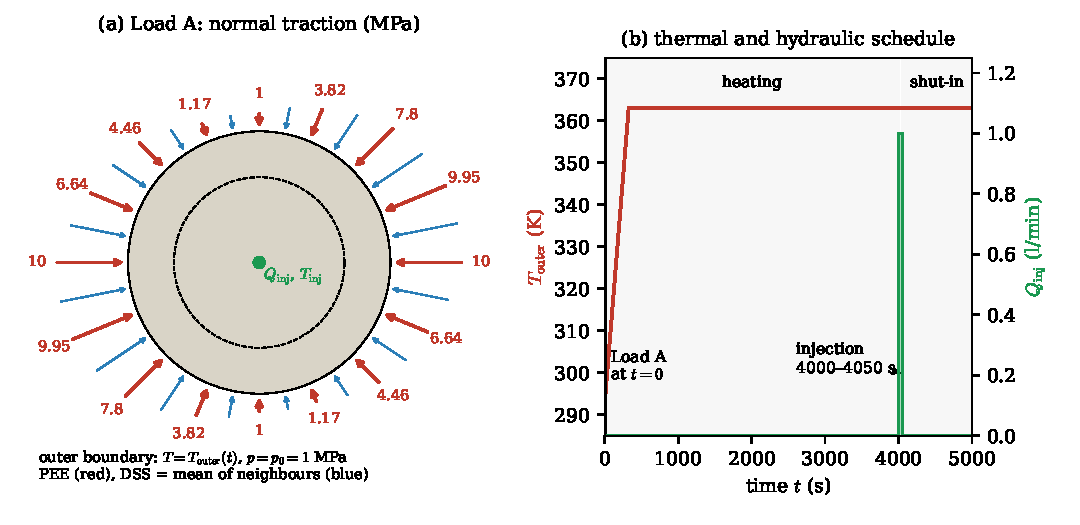
\includegraphics[width=\textwidth]{fig_bc.pdf}
\caption{THM2 boundary conditions: Load~A tractions (a) and the thermal and
hydraulic schedule (b).}
\label{fig:bc}
\end{figure}

\textbf{Initial state:} $T_0=\SI{293}{K}$, $p_0=\SI{1}{MPa}$, $\mathbf u=\mathbf 0$
everywhere. Initial effective stress $\alpha_B p_0$ in the rock (0 in the
sheath), so that total stress is zero before loading. Report strains relative to
this state.

\textbf{Boundaries:} the outer boundary is drained ($p=p_0$) and has the
prescribed temperature in all phases. The reference model treats the sheath
hydraulically and thermally like the rock.

\textbf{Time stepping (reference):} \SI{5}{s} to \SI{400}{s}, \SI{40}{s} to
\SI{4000}{s}, \SI{1}{s} during injection, \SI{2}{s} to \SI{4150}{s}, \SI{10}{s}
to \SI{5000}{s}. Teams may use other steps but must hit all output times exactly.

% ---------------------------------------------------------------
\section{Required outputs}
\label{sec:outputs}
% ---------------------------------------------------------------
Each team delivers four CSV files per rock and load case, in SI units,
comma-separated, with one header line (Table~\ref{tab:outputs}). File names
follow \texttt{<team>\_<case>\_<rock>\_load<X>\_<output>.csv}, e.g.\
\texttt{UFZ\_THM2\_greywacke\_loadA\_probe.csv}.

\begin{table}[htbp]
\centering
\caption{Required output files.}
\label{tab:outputs}
\small
\begin{tabularx}{\textwidth}{@{}lLLL@{}}
\toprule
Output & Location & Times & Columns \\
\midrule
\texttt{centre}  & Centre point $(0,0)$ & Every time step, at least every 5\,s; every 1\,s in 4000--4060\,s & \texttt{t, T, p} \\
\texttt{probe}   & Probe circle $r=\SI{0.065}{m}$, 360 points at \ang{1} & Output times & \texttt{t, theta\_deg, eps\_xx, eps\_yy, eps\_xy, eps\_vol, eps\_tt, T, p} \\
\texttt{profile} & Radial line $\theta=\ang{0}$, $0\le r\le\SI{0.1}{m}$, 101 points & Output times & \texttt{t, r, T, p, sigma\_rr, sigma\_tt} \\
\texttt{mean}    & Probe circle average & Every time step & \texttt{t, eps\_vol\_mean, T\_mean, p\_mean} \\
\bottomrule
\end{tabularx}
\end{table}

\textbf{Output times:} 5, 325, 2000, 4000, 4001, 4005, 4010, 4025, 4050, 4060,
4100, 4200, 4500, 5000\,s. For M1 only the state after loading is required
($t=\SI{5}{s}$ or the end of the mechanical step).

\textbf{Sign convention:} tension positive for stress and strain in the output
files (the PEE loads above are given as compression positive).
$\varepsilon_\mathrm{vol}=\varepsilon_{xx}+\varepsilon_{yy}$;
$\varepsilon_{\theta\theta}$ (\texttt{eps\_tt}) is the circumferential strain,
comparable with the fibre-optic measurement.

Teams also submit a short model description: code and version, process
formulation, element type, mesh size and node count, time stepping, and any
deviation from this specification.

% ---------------------------------------------------------------
\section{Verification checks}
\label{sec:verification}
% ---------------------------------------------------------------
Each team should pass the checks in Table~\ref{tab:checks} before submitting;
reference values are from the OGS~6.5.9 model.

\begin{table}[htbp]
\centering
\caption{Verification checks and reference values ($\varepsilon_\mathrm{vol}$ in $10^{-2}$\,\%).}
\label{tab:checks}
\small
\begin{tabularx}{\textwidth}{@{}lLLLl@{}}
\toprule
Check & Quantity & Reference (OGS) & Independent check & Target \\
\midrule
T: ramp only & $T(r,t)$ & -- & Duhamel solution, disc $R=\SI{0.1}{m}$ & $\le$ 0.2\,K \\
Heating   & Centre $T$ at 4000\,s & 356.7\,K & T model & $\le$ 0.5\,K \\
Injection & $p-p_0$ at $r=\SI{0.065}{m}$ & 0.0812\,MPa & Thiem: 0.0811\,MPa & $\le$ 1\,\% \\
Injection & $p-p_0$ at centre node & 1.12\,MPa & Mesh-dependent & Report only \\
Cooling   & Centre $T$ at 4100 / 5000\,s & 309.5 / 353.6\,K & -- & $\le$ 1\,K \\
M1        & Mean $\varepsilon_\mathrm{vol}$ on probe circle & $-2.46$ (Greywacke), $-0.95$ (Gneiss) & -- & $\le$ 2\,\% \\
Heating   & Mean $\varepsilon_\mathrm{vol}$ at 4000\,s & 11.15 (Greywacke), 12.03 (Gneiss) & $2(1+\nu)\alpha_T\Delta T+\varepsilon_\mathrm{mech}$, $\Delta T=\SI{67.0}{K}$ & $\le$ 2\,\% \\
Injection & Min.\ mean $\varepsilon_\mathrm{vol}$ after injection & 10.73 at 4460\,s (Greywacke), 11.62 at 4450\,s (Gneiss) & -- & Report \\
Recovery  & Mean $\varepsilon_\mathrm{vol}$ at 5000\,s & 10.94 (Greywacke), 11.82 (Gneiss) & -- & $\le$ 2\,\% \\
\bottomrule
\end{tabularx}
\end{table}

The strain on the probe circle varies with angle, with maxima near \ang{100}
and \ang{280} under Load~A. Temperature and pressure are the same for both
rocks, because permeability and bulk thermal properties are equal.

% ---------------------------------------------------------------
\section{Modelling choices and open items}
\label{sec:open}
% ---------------------------------------------------------------
Teams must state how they handle the following, since the specification leaves
them open or the reference model uses a simplification:
\begin{itemize}
  \item \textbf{Coupling scheme:} monolithic or staggered; convergence tolerances.
  \item \textbf{Mass vs.\ volume balance:} with pressure-dependent water
        density, injection is a mass rate (\SI{16.67}{g\,s^{-1}} per m).
  \item \textbf{Point injection:} source at a node vs.\ resolved borehole;
        pressure at the injection point is mesh-dependent.
  \item \textbf{Thermal mixing rule} used to reach the prescribed bulk
        $\lambda$ and $\rho c$.
\end{itemize}

Open items for the task group:
\begin{itemize}[label=\open]
  \item Sheath permeability: the paper gives \SI{1e-19}{m^2}; the reference
        uses rock permeability to keep a drained outer boundary. Agree on one
        choice.
  \item Measured PEE and DSS arc widths (currently \ang{18}/\ang{4.5} estimates).
  \item Injection rate per metre in 2D vs.\ the \SI{0.2}{m} sample height in
        the experiment.
  \item Thermal expansion coefficient of the rocks (\SI{8e-6}{K^{-1}} assumed)
        and of water (neglected).
  \item Fractured cases (HM3, HM4, THM3, THM4): fracture properties, aperture
        law, injection into the fracture.
  \item Agree output formats and file naming proposed in Section~\ref{sec:outputs}.
  \item Comparison data from GREAT cell heating tests and fibre-optic strain.
\end{itemize}

% ---------------------------------------------------------------
\nocite{McDermott2018,Kolditz2025,Mollaali2026}
\bibliographystyle{unsrtnat}
\bibliography{../references}

\end{document}
